\section*{Hybrid: 3 (smaller) page tables per process}
\begin{minipage}{0.5\linewidth}
  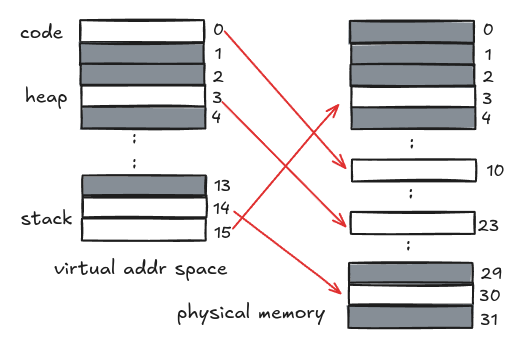
\includegraphics[width=\linewidth]{imgs/bigger_sparse_page}
\end{minipage}
\begin{minipage}{0.5\linewidth}
  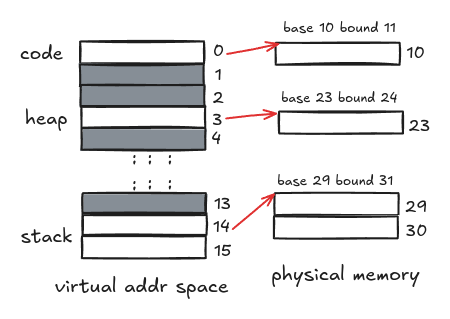
\includegraphics[width=\linewidth]{imgs/hybrid_page_table}
\end{minipage}
\begin{itemize}
\item each proc has \emph{three} associated page tables (right) instead of one (left)
\item each logical seg has 3 pairs of base/bound (hardware) regs: base points to the page table addr; bound shows page table size
\item use 2 bits for segment (e.g. 00 unused, 01 code, 10 heap, 11 stack)
\end{itemize}
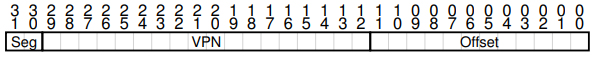
\includegraphics[width=\linewidth]{imgs/virtual_addr2_32big_hybrid}
\begin{minipage}{0.61\linewidth}
\begin{lstlisting}[language=c,xrightmargin=2pt]
SN = (VirtualAddr & SEG_MASK) >> SN_SHIFT
VPN = (VirtualAddr & VPN_MASK) >> VPN_SHIFT
AddrOfPTE = Base[SN] + (VPN * sizeof(PTE))
\end{lstlisting}
\end{minipage}
\begin{minipage}{0.39\linewidth}
  \flushleft
  \begin{itemize}
  \item \emph{bound} reg to decide how many pages to map
  \item SN (seg num) to decide which base/bound pair
  \end{itemize}
\end{minipage}
\begin{itemize}
\item not flexible: segmentations still assume usage patterns (separation of code/stack/heap in allocating pages)
\item \textbf{external fragmentation} While most of memory is managed in page-sized units, page tables now of arbitrary size (in multiples of PTEs). Thus, finding free space for them in memory is more complicated
\end{itemize}
